% !TEX root = ../main.tex 

\section{Defining Mechanistic Staiblity}
At the highest level, \textit{mechanistic stability} is the stability
of a model's decision criteria with respect to changes in the input.
In many cases, we expect a strong, generalizable learner to also be
one that is mechanistically stable. For example, given two-operand
addition problems, we would expect a strong learner to add four-digit
numbers in the same way it adds eight-digit numbers. On the other
hand, a mechanistically stable learner may be necessary for fairness.
Consider a model that evaluates job applicants. A legal and ethical model
must not change its evaluation criteria based on an applicant's gender. 
In this paper, we formalize using tools from category theory, this notion
of mechanistic stability. Then, we show that mechanistic stability is a
sufficient condition for both generalization and robustness. Finally, we
provide a host of empirical results to showcase when mechanistic stability
can be induced or inhibited. Throughout the paper, we use the task of 
two-operand addition as a running
example.

This remainder of this section is organized as follows:
\begin{enumerate}
\item First, in Section~\ref{s:partitioning-subtasks}, we formalize 
what we mean by ``changes in the input'' through
the concept of a \textit{permissible partition} over a data distribution.
\item Then, in Section~\ref{s:causal-equiv}, we define ``stability a model's decision criteria'' through
a category-theoretic equivalence between a model's mechanism on a specific
\textit{permisssible partition}. 
\item FInally, in Section~\ref{s:mech-stab}, by combining these components 
together, we arrive at our
notion of \textit{mechanistic stability}.
\end{enumerate}

Our contribution focuses on the supervised learning regime. Under this setup,
any model's input is chosen from a set $\cX$ and its outputs lie in a set
$\cY$. Let $(\cX, \cF_\cX, \P_\cX)$ and $(\cY, \cF_\cY, \P_\cY)$ be
probability spaces over $\cX, \cY$, respectively. 
Denote by $(\cX \times \cY,
\cF_\cX \otimes \cF_\cY, \P_\cX \times \P_\cY)$ the product probability
space over all input-output pairs. We call any probability measure 
$\P_{\cX\times\cY}$ that is absolutely continuous\footnote{For any
$E \in \cF_\cX\otimes \cF_\cY$, if $(\cP_\cX \times \cP_\cY)(E) = 0$,
then $\P_{\cX\times\cY}(E) = 0$.} to 
$\P_\cX \times \cP_\cY$ a \textit{data distribution}. A data distribution
also determines the conditional distribution $\cP_{\cX\times\cY}[y | x]$
which intuitively captures the elements of $\cY$ that are an appropriate
response given $\cX$. Therefore, any supervised learning task can be 
seen as learning the distribution $\cP_{\cX\times\cY}$. 
\begin{defn}[Task]\label{d:task}
A \textbf{task}, $T$, is a data distribution which we also denote as
$\cD$.
\end{defn}
For the remainder of the paper, our discussions resolve around a \textit{
single, fixed, but arbitrary}
 task.  A brief discussion on the generalizations of
this concept to the multitask setting can be found in ...
Moreover, we use $T, \cD, \P_{\cX\times\cY}$ interchangably.

\subsection{Partitioning Subtasks}\label{s:partitioning-subtasks}
Many tasks contain inherent structure. For two-operand addition, we can
divide this tasks into \textit{subtasks}, where each subtask is the
set of all $m$-by-$n$ digit addition problems. Herein, we formalize
this notion of task substructure through \textit{subtasks}. To do
this, we partition the universe of all possible input-outputs through a 
\textit{permissble partitioning}.
\begin{defn}[Permisslbe Partition]\label{d:permissible}
For a given task $T$ with distribution $\cD$, a \textbf{permissible partition},
denoted by $\cS$, is a countable collection of measurable subsets of 
$\cF_\cX\otimes \cF_\cY$ that satisfies
\begin{align}
s' \cap s &= \emptyset \qquad \text{for all}~s,s' \in \cS,\\
\bigcup_{s\in \cS} s &= \cX \times \cY, \\
\P_{\cX\times\cY}[s] &> 0 \qquad \text{for all}~s \in \cS.
\end{align}
\end{defn}
Henceforth, unless otherwise specified, we assume that all partitions are 
permissible. A partitions not only carves up $\cX \times \cY$ but also
induces two new types of distributions. These are shown and expanded upon
in Fig.~\ref{f:permissible-partition-induced-distributions}.

\begin{figure}[h!]
\centering
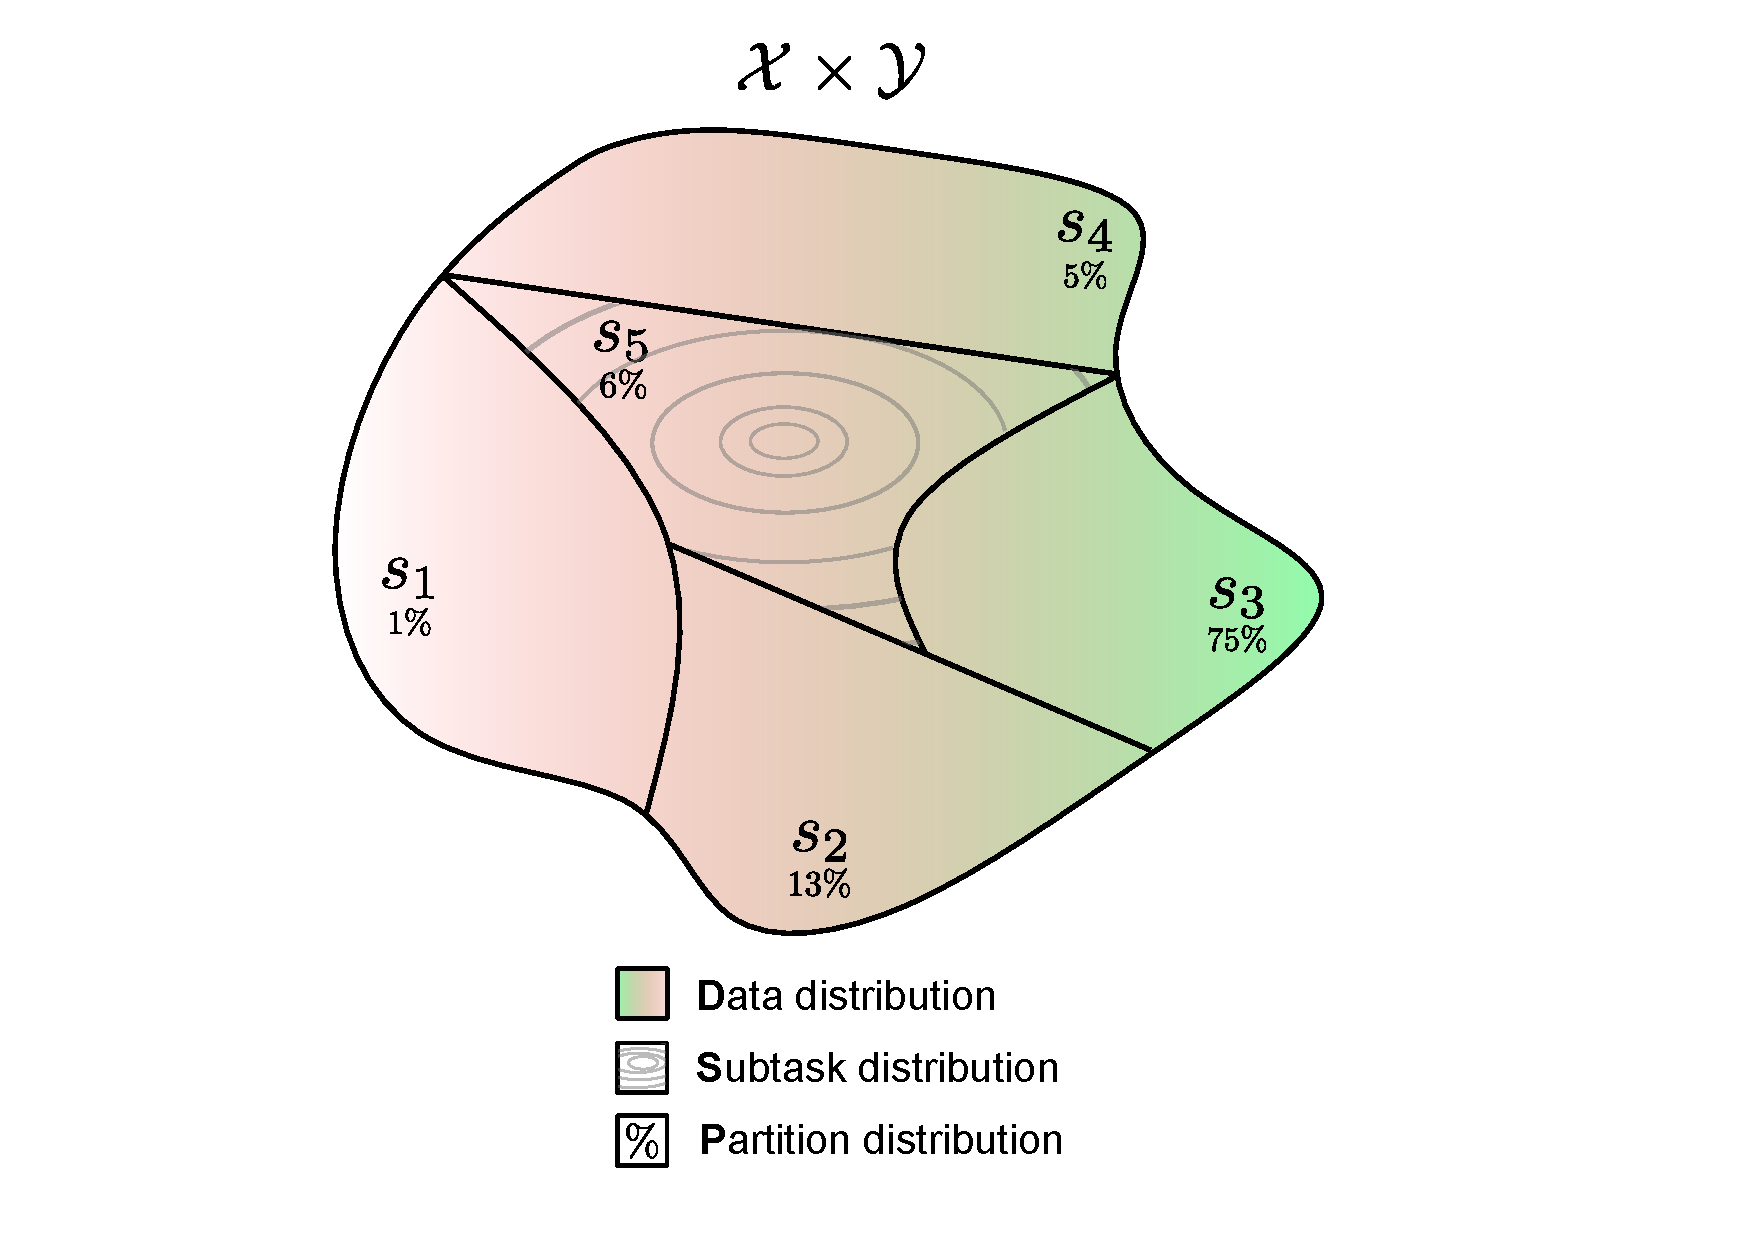
\includegraphics[width=0.5\textwidth]{figs/permissible-partition.pdf}
\caption{Starting with a data distribution $\cD$, a partition
induces two additional distributions of interest: subtask distributions
(\textbf{S}), and the partition distribution (\textbf{P}). 
The underlying data
distribution of the task (\textbf{D}) is shown as a color gradient
and behaves independent of any partition. 
On the other hand, the subtask
distribution (\textbf{S}) is the data distribution conditional 
on a particular
element of the partition. Lastly, the partition distribution 
represents the probability that an input-output pair drawn from
\textbf{D} will fall in any element of the partition.}
\label{f:permissible-partition-induced-distributions}
\end{figure}
By Def.~\ref{d:permissible}, since any element of a partition
has non-zero probability mass, the data distribution conditioned on this
element is well-defined and is itself also a data distribution 
(see Def~\ref{d:task}). Thus, we can now formally define the notion
of a \textit{subtask}.
\begin{defn}[Subtask]
For a given task, $T$, and its corresponding data distribution 
$\P_{\cX\times\cY}$, consider any partition $\cS$ of $T$.
For any $s \in \cS$, a \textbf{subtask}, $T_s$, is the conditional
distribution
\[
\P_{\cX\times \cY | s}[A] = \P_{\cX\times \cY}[A | s]
= \frac{\P_{\cX\times\cY}[A \cap s]}{\P_{\cX \times \cY}[s]}.
\]
This last equation is the definition of conditional probability.
When it is clear from context what the partition is 
we denote this distribution as $\P_s$.
\end{defn}
For any partition, we also define a discrete \textit{partition distribution}
that will come in use technically in a bit. 
\begin{defn}\label{d:partition-distribution}
For a given task $T$, parition $\cS$, the \textbf{partition distribution}
is a probability space $(\cS, 2^{\cS}, \P_\cS)$, where for all $s \in \cS$,
$\P_\cS[s] = \P_{\cX\times\cY}[s]$.
\end{defn}

% I'm not sure if taking the powerset here is ok, in particular, we need
% to make sure that this powerset sigma-algebra is a subset of the product
% sigma-algebra that was defined earlier.

\begin{rmk}
The conditions for a partition to be permissible is quite weak. Are there
perhaps more desirable conditiosn that we should require out permissble
partitions to have? Fundamentally, as the partitions get larger and larger,
it should be easier to achieve mechanistic stability. Some things to think
about:
\begin{itemize}
\item Changing ``countable collection'' to a ``finite collection''?
\item Instead of only requiring that our partitions have positive
probability mass, maybe we need that the subsets be $\eps$-representative
\citep{shalev-shwartz_understanding_2014}.
\end{itemize}
\end{rmk}

\subsection{Causal Equivalence: A Category-Theoretic Perspective}
\label{s:causal-equiv}
Herein, we introduce some basic category-theoretic concepts and use them
to formally define causal graphs and their equivalence,. These constructions
originate from~\cite{jacobs_causal_2021} and have since been expanded upon
through works such as~\cite{beckers_abstracting_2019,{}
otsuka_equivalence_2022,zennaro_abstraction_2022,massidda_causal_2023}
have extended this framework for their own specific
applications. We provide a brief introduction here and refer the reader
to both~\cite{jacobs_causal_2021} for the detailed constructions. 

\begin{defn}
Let $\textsf{Stoch}$ be the category of all probability spaces. Its objects
are probability spaces and its morphisms are Markov transition kernels\footnote{
One can find a detailed construction \href{https://arxiv.org/pdf/2111.13837}
{here}. This is an extension of the framework presented in \cite{jacobs_causal_2021}
as they only consider the construction of \textsf{Stoch} with finite sets and
transition matrices.}.
\end{defn}
A causal graph not only contains the probability dynamics between its variables
(the semantics of the causal graph), but it also contains syntactical information
that encode real-world knowledge a priori restricting the set of permissible
probability transition dynamics. We can also define a category that captures
these structures.
\begin{defn}
Let $G = (V_G, E_G)$ be a directed acyclic graph (DAG) with vertices $V_G$ and edges
$E_G$. Denote by $\textsf{Syn}_G$ be the free $\textsf{CDU}$ category\footnote{
for a detailed construction of this see \cite{jacobs_causal_2021}.
} generated
by $G$. 
\end{defn}
Both $\textsf{Stoch}$ and $\textsf{Syn}_G$ are \textit{symmetric monoidal categories}. 
We are now ready to formally define a causal graph.
\begin{defn}
A \textbf{causal graph} defined by the DAG $G$, is a functor $F: \textsf{Syn}_G \to
\textsf{Stoch}$.
\end{defn}
Next is a result from~\cite{jacobs_causal_2021} which shows that we haev in some
sense sufficiently captured the set of all causal graphs.
\begin{prop}
There is a 1-1 correspondance between the Bayesian networks on a DAG $G$ and
the functors of type $\textsf{Syn}_G \to \textsf{Stoch}$.
\end{prop}
We then directly use this category-theoretic notion of causality to define equivalence
between two causal models on the same causal graph which is a special case of
causal-equivalence defined in~\cite{otsuka_equivalence_2022}.
\begin{defn}
Let $F, H: \textsf{Syn}_G \rightrightarrows \textsf{Stoch}$ be two causal graphs
on $G$. Then, $F, H$ are \textbf{causally-equivalent} if there exists a natural
isomorphsim from $F$ to $H$. 
\end{defn}
For any model $M$, we may consider its mechanisms to be a causal graph,
a functor from $\textsf{Syn}_M \to \textsf{Stoch}$. Moreover, for two
distinct subcircuits/submechanisms of the same model, we can model them
as parallel functors $\textsf{Syn}_M \rightrightarrows \textsf{Stoch}$.

\subsection{Mechanistic Stability}\label{s:mech-stab}
With these notions of causal equivalence defined in the previous section,
we are now ready to define mechanisitic stability.

\begin{defn}[$\eps$-Mechanistically Stable]
A model $M$ is $\eps$-mechanistically stable for any $\eps > 0$ with respect
to some task $T$, if 
\begin{equation}
\sup_{\cS:\text{partition}}
\left[\P_{s, s' \sim \cS \otimes \cS}[F_s \not\cong F_{s'}]\right] < \eps,
\end{equation}
where $\P_{s,s'}$ is the measure on the product partition space\footnote{
sampling two partitions at randomly according to the partition distribution
defined in Def.~\ref{d:partition-distribution}.
}, $F_s$ is the causal graph induced by the subtask distribution $s$ and
$F_s \not \cong \F_{s'}$ denotes that the causal graphs $F_s, F_{s'}$ are not
causally equivalent.
\end{defn}

